\documentclass[11pt,letterpaper]{article}
\usepackage[T1]{fontenc}
\usepackage[utf8]{inputenc}
\usepackage[margin=0.94in,headheight=15pt]{geometry}
\usepackage{amsmath,amsthm,mathtools,newtxtext,newtxmath}
\usepackage{microtype,booktabs,array,tabularx,longtable,enumitem}
\usepackage{xcolor,tikz,fancyhdr,titlesec,needspace,placeins}
\usepackage{algorithm,algpseudocode,fontawesome5,xurl,hyperref}
\usetikzlibrary{arrows.meta,positioning,calc,fit}
\definecolor{ink}{HTML}{35204D}
\definecolor{muted}{HTML}{655B71}
\definecolor{pale}{HTML}{F4F1F8}
\hypersetup{colorlinks=true,linkcolor=ink,citecolor=ink,urlcolor=ink,
 pdftitle={Out-Learn: Change What You Need to Know},pdfauthor={Vincent Boucher},
 pdfsubject={Constructed experiments, sharp calibration guarantees, and reusable learning interfaces}}
\urlstyle{same}
\pagestyle{fancy}\fancyhf{}
\fancyhead[L]{\small\textsc{Out-Learn}}
\fancyhead[R]{\small Boucher / MONTREAL.AI}
\fancyfoot[C]{\thepage}\renewcommand{\headrulewidth}{.3pt}
\setlength{\parindent}{1.1em}\setlength{\parskip}{.15em}
\setlength{\emergencystretch}{2em}\renewcommand{\arraystretch}{1.14}
\setlist{nosep,leftmargin=1.5em,topsep=.3em}
\titleformat{\section}{\large\bfseries\color{ink}}{\thesection}{.6em}{}
\titleformat{\subsection}{\normalsize\bfseries}{\thesubsection}{.6em}{}
\titlespacing*{\section}{0pt}{1.1em}{.5em}
\titlespacing*{\subsection}{0pt}{.75em}{.3em}
\newcolumntype{Y}{>{\raggedright\arraybackslash}X}
\newcolumntype{P}[1]{>{\raggedright\arraybackslash}p{#1}}
\newcommand{\RR}{\mathbb R}\newcommand{\NN}{\mathbb N}
\newcommand{\calV}{\mathcal V}\newcommand{\calP}{\mathcal P}
\newcommand{\norm}[1]{\lVert#1\rVert}
\newcommand{\Om}{SUCCESSOR~$\Omega$}
\newcommand{\thesis}[1]{\begin{center}\setlength{\fboxsep}{9pt}\fcolorbox{ink}{pale}{\begin{minipage}{.92\linewidth}#1\end{minipage}}\end{center}}
\DeclareMathOperator{\dist}{dist}\DeclareMathOperator{\clip}{clip}\DeclareMathOperator{\sgn}{sgn}
\newtheorem{theorem}{Theorem}[section]
\newtheorem{proposition}[theorem]{Proposition}
\newtheorem{lemma}[theorem]{Lemma}
\newtheorem{corollary}[theorem]{Corollary}
\theoremstyle{definition}\newtheorem{definition}[theorem]{Definition}
\theoremstyle{remark}\newtheorem{remark}[theorem]{Remark}
\renewcommand{\topfraction}{.95}\renewcommand{\bottomfraction}{.85}
\renewcommand{\textfraction}{.06}\renewcommand{\floatpagefraction}{.8}
\pdfinfoomitdate=1
\pdftrailerid{}
\begin{document}
\thispagestyle{plain}
\begin{center}
{\small\sffamily\color{ink} MONTREAL.AI\quad /\quad TRANSFORMATIONAL INTELLIGENCE $\infty$}\par
\vspace{1.05em}
{\fontsize{35}{39}\selectfont\bfseries\color{ink} Out-Learn\ \raisebox{.12ex}{\Large\faBookOpen}\par}
\vspace{.45em}
{\Large\bfseries Change What You Need to Know\par}
\vspace{.5em}
{\large Constructed Experiments and Sharp Calibration Guarantees\par}
{\large for Reusable Learning\par}
\vspace{1em}
{\large Vincent Boucher\par}
MONTREAL.AI\par
Montr\'eal, Qu\'ebec, Canada\par
\vspace{.5em}
21 October 2026\quad$\cdot$\quad Revised research manuscript
\end{center}
\begin{abstract}
A learner can identify hidden conditions, or construct an experiment whose answer no longer depends on them. The first Out-Learn manuscript selected between observations and supplied interfaces in a finite world catalogue. This revision constructs the measurement protocol itself and learns its calibration from numerical observations. The new setting has an unknown continuous gain, arbitrary response functions, and polynomial drift whose unrestricted coefficients can change in every measurement block. We synthesize sampling times, polarity changes and correction weights, rather than supply a finished drift-rejecting interface. Norm duality gives an exact error limit against every decoder. A sparse-construction theorem reduces the least-cost known-gain problem to $d+2$ readings for degree-$d$ drift; a zero-transcript argument shows that deterministic adaptation cannot lower its worst acquisition cost under the stated architecture. For an unknown positive gain, we derive a sharp joint calibration--use minimax law, with two different underlying signals producing identical complete raw observations. That law couples the experiment used to learn the gain to the number of future uses. In an exact synthetic quadratic-drift study, the least-cost one-use pair costs thirteen declared resource units and guarantees error $3/1003$. A different calibration becomes optimal beyond nineteen uses. The frozen interface supports adaptive queries and two downstream decision problems; a scope-changing successor retains valid gain evidence but replaces its measurement program. The earlier finite study is preserved and reproduced. The contribution is a completed experiment-construction and learning contract, not new physical primitives, a model-free learner, or an established business.
\end{abstract}
\noindent\textbf{Keywords:} transformational intelligence; experimental design; optimal recovery; calibration; nuisance rejection; reusable capability; SUCCESSOR $\Omega$.
\begin{center}\small
\textbf{Find your Alpha. Build your SUCCESSOR $\Omega$.}\par
\href{https://github.com/MontrealAI/AGI-Alpha-Agent-v0}{github.com/MontrealAI/AGI-Alpha-Agent-v0}
\end{center}
\clearpage

\section{The next lesson can be a better experiment}
A learning system receives a drifting measurement. It could fit a richer model, acquire more samples, or ask more capable agents to reconstruct the drift. It could also change the sequence of physical operations so that the unwanted dependence cancels before the scientific answer is inferred.

The difference is not rhetorical. Without an informative change of measurement, two different signals can produce the same complete observations. No decoder can distinguish them. With an appropriate constructed sequence, a bounded-error answer can be available even though the drift coefficients remain unreported and may change completely at the next use.

\thesis{\textbf{Do not only improve the model that explains the measurement. Construct the experiment that makes an unnecessary explanation disappear.}\par\smallskip
Learn the calibration that remains necessary. Retain the protocol and the evidence that make the next investigation possible.}

This revision applies that principle to its own predecessor. The first \emph{Out-Learn} paper supplied a partial bypass with a known correctness contract, then synthesized when to buy it and which observation to make \cite{original}. Its finite continuation theorem is useful and is preserved. But the trusted component doing the decisive work was already in the catalogue. Here the output is instead an executable measurement schedule, its correction coefficients, a calibration interval obtained from observations, and an error certificate for subsequent queries. The input still includes primitive semantics and a structural model class; those assumptions are not disguised as discoveries.

\subsection{One experiment a reader can check}
Let an unknown response $f$ be observed through an unknown positive gain $g$ and arbitrary quadratic drift:
\begin{equation}
 y_i=g\sigma_i f+\theta_0+\theta_1t_i+\theta_2t_i^2+e_i.
 \label{eq:opening}
\end{equation}
A polarity command $\sigma_i\in\{-1,1\}$ changes the signal's sign while preserving its intended meaning. The drift coefficients are unknown. They need not be the same in the reference measurement and the later scientific measurement.

For a declared cost of reading, switching and waiting, the compiler chooses
\begin{equation}
 (t_i)=(0,2,3,5),\qquad(\sigma_i)=(+,+,-,-),\qquad
 w=\tfrac18(-1,5,-5,1).
 \label{eq:primaryword}
\end{equation}
The resulting contrast is
\begin{equation}
 z=\frac{-y_0+5y_2-5y_3+y_5}{8}=gf+w^Te,
 \label{eq:openingcontrast}
\end{equation}
because the weights annihilate $1,t,t^2$ and preserve the signed signal. The first positive-polarity reading has a negative correction weight: simply averaging by polarity would not implement this experiment.

Measure a unit reference through its own block, giving contrast $c=g$ in the noiseless case. Then $z/c=f$, without first reconstructing either block's nuisance polynomial. Table~\ref{tab:opening} is an executed rational example, not a field measurement. Its two drifts are $11+t+2t^2$ and $3-2t+t^2$; its gain is $7/5$ and its intended response is $2/7$.

\begin{table}[htbp]\centering\small
\caption{A constructed protocol, two different unknown drifts, one recovered response. The nuisance values are revealed to the independent checker, not supplied to the decoder.}
\begin{tabular}{@{}lrrrrc@{}}\toprule
 & $t=0$ & $t=2$ & $t=3$ & $t=5$ & Corrected contrast\\\midrule
Polarity & $+$ & $+$ & $-$ & $-$ & \\
Unit-reference readings & $62/5$ & $112/5$ & $153/5$ & $323/5$ & $c=7/5$\\
Unknown-response readings & $17/5$ & $17/5$ & $28/5$ & $88/5$ & $z=2/5$\\\bottomrule
\end{tabular}\par\smallskip
\textbf{Recovered response: $z/c=2/7$.}
\label{tab:opening}
\end{table}

The noiseless cancellation is classical measurement mathematics. The substantive questions developed here are harder: what error is unavoidable with bounded raw errors, which sequence is least costly at an accepted precision, how much to invest in calibration before repeated use, and which part of a learned capability survives an expanded nuisance class?

\subsection{The precise advance, without renaming prior art}
Drift-eliminating comparison designs, sign reversal and polynomial rejection have substantial metrological precedent \cite{doiron,swanson}. Optimal recovery already studies best possible reconstruction from bounded-error observations \cite{ettehad}. The present contribution is not that subtraction removes an offset, that a polynomial has a finite-dimensional representation, or that experiments should serve a purpose.

Three results carry the revision: exact sparse experiment construction, a sharp calibration--use law against every decoder, and a reuse-sensitive choice of what to calibrate. The code returns programmes, learns calibration from raw readings, exports intervals and repairs a changed scope. Section~\ref{sec:lineage} preserves the original finite learner at its original strength.

The research target is a reusable capability: \emph{an experiment that can make an entire family of unknown response functions accessible under a declared error requirement}. It is not an assertion that every real nuisance is polynomial or that the compiler discovers new physics.

\section{What can change, and what must remain true}
\label{sec:model}
\subsection{A continuous uncertainty class}
A measurement block holds an intended response $s=f(x)\in[-S,S]$ constant while sampling distinct increasing slots from a finite time grid $\mathcal T$. Its data are
\begin{equation}
 y=g\sigma s+V_d(t)\theta+e,\qquad
 (V_d(t))_{ik}=t_i^k\ (k=0,\ldots,d),\qquad |e_i|\le\eta.
 \label{eq:model}
\end{equation}
Here $S>0$, $g\ge g_0>0$, and $\theta\in\RR^{d+1}$ is unrestricted. Gain is stable within the reference/use scope. The polynomial coefficients may vary freely between blocks. The unknown response $f$ may be nonlinear, and later inputs may depend on earlier reported answers. No list of possible numerical gains, coefficients or response values is supplied to the constructor.

The programme is finite because the \emph{action grammar} is finite, not because the possible worlds are enumerated. The code searches time subsets and signs. It does not search a finite list of true polynomial coefficients or precomputed response tables. The exact rational simulator chooses some values only after the programme has been constructed.

The following obligations give the model scientific meaning. Reversal must multiply the desired signal by the commanded sign without changing its scientific definition. Within a block, the intended response must remain constant. The non-signal contribution must lie in the declared polynomial space plus the raw-error budget. A known unit reference must genuinely have response one. Sensor range, timing and modulation errors must fit the qualified assumptions. Neither algebra nor a successful synthetic test establishes those conditions in hardware.

\subsection{An executable interface rather than a learned label}
A constructed programme is
\begin{equation}
 P=(t,\sigma,w,A,c_P),\qquad
 w^T\sigma=1,\quad w^TV_d(t)=0,\quad A=\norm{w}_1.
 \label{eq:program}
\end{equation}
It returns $z=w^Ty$ with $|z-gs|\le\eta A$. Its declared acquisition cost is
\begin{equation}
 c_P=n c_{
m read}+\nu(\sigma)c_{
m switch}+t_n c_{
m time},
 \label{eq:cost}
\end{equation}
where $\nu$ counts polarity changes \emph{between retained readings}, $c_{
m read}>0$, and the other prices are nonnegative. The clock starts at zero. Distinct slots and sequential acquisition are architectural restrictions; simultaneous opposite-polarity channels are a different comparison.

There is no uncharged restoration between blocks. If the modulator's known current polarity is $h\in\{-1,1\}$, execute the normalized programme with actual signs $h\sigma$ and return $hw^Ty$. Its final polarity is inherited by the next block. Thus normalizing the first sign to positive costs no reset. Initialization and qualification are common supplied resources, not assumed free physical services.

For the uniform integer grid $\{0,\ldots,T\}$, translating a schedule to start at zero preserves the polynomial space and does not increase waiting cost. If moving the start would violate a real warm-up or availability constraint, that reduction is no longer licensed. Such conditions must enter the grammar rather than disappear from the ledger.

\begin{figure}[htbp]\centering
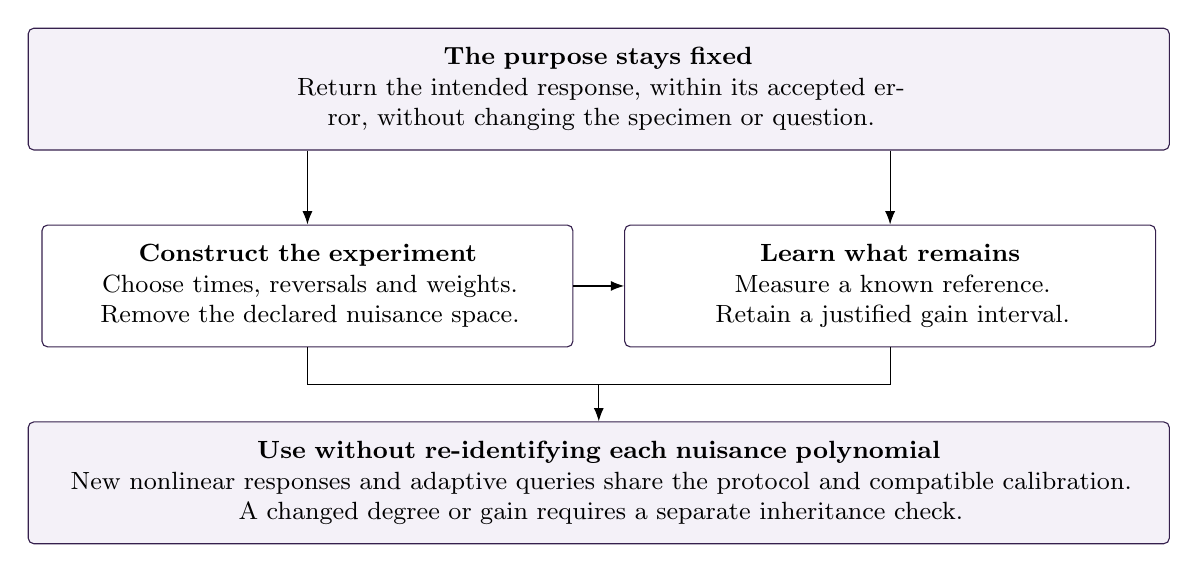
\begin{tikzpicture}[>=Latex,font=\small,
 box/.style={draw=ink,rounded corners=2pt,align=center,inner sep=7pt}]
\node[box,fill=pale,text width=14cm] (purpose) at (7,0) {\textbf{The purpose stays fixed}\par Return the intended response, within its accepted error, without changing the specimen or question.};
\node[box,text width=6.25cm] (construct) at (3.3,-2.5) {\textbf{Construct the experiment}\par Choose times, reversals and weights.\par Remove the declared nuisance space.};
\node[box,text width=6.25cm] (learn) at (10.7,-2.5) {\textbf{Learn what remains}\par Measure a known reference.\par Retain a justified gain interval.};
\draw[->] (purpose.south -| construct.north)--(construct.north);
\draw[->] (purpose.south -| learn.north)--(learn.north);
\draw[->] (construct.east)--(learn.west);
\node[box,fill=pale,text width=14cm] (uses) at (7,-5.0) {\textbf{Use without re-identifying each nuisance polynomial}\par New nonlinear responses and adaptive queries share the protocol and compatible calibration.\par A changed degree or gain requires a separate inheritance check.};
\draw[-] (construct.south)--(3.3,-3.75)--(10.7,-3.75)--(learn.south);
\draw[->] (7,-3.75)--(uses.north);
\end{tikzpicture}
\caption{The learner changes the observation process, then learns a numerical calibration. Primitive preservation and drift-class assumptions remain supplied; the programme, correction and evidence-dependent intervals are outputs.}
\label{fig:learning}
\end{figure}

\section{The exact information carried by a programme}
\label{sec:quotient}
\subsection{A geometric quantity with an operational meaning}
For fixed times and signs, let $\calV=\operatorname{col}V_d(t)$ and define
\begin{equation}
 \kappa(t,\sigma)=\dist_\infty(\sigma,\calV),\qquad
 A_*(t,\sigma)=\min\{\norm{w}_1:w^T\sigma=1,\ w\perp\calV\}.
 \label{eq:kappa}
\end{equation}
The minimum is infinite if no such contrast exists. Signal and nuisance are indistinguishable precisely when $\kappa=0$. Otherwise the usual finite-dimensional norm duality gives $A_*=1/\kappa$. The two objects have different uses: a weight vector certifies an achievable error; a nearby nuisance polynomial certifies why no decoder can do better.

\Needspace{9\baselineskip}
\begin{theorem}[Exact known-gain recovery radius]
\label{thm:known}
Fix a known $g>0$, $|s|\le S$, unrestricted $v\in\calV$ and $\norm{e}_\infty\le\eta$ in $y=g\sigma s+v+e$. If $\kappa>0$, the smallest worst absolute error over \emph{all} reconstruction maps is
\begin{equation}
 \inf_D\sup_{s,v,e}|D(y)-s|=
 \min\left\{S,\frac{\eta}{g\kappa}\right\}
 =\min\left\{S,\frac{\eta A_*}{g}\right\}.
 \label{eq:knownradius}
\end{equation}
If $\kappa=0$, the radius is $S$, even with zero noise. No linearity restriction is imposed on $D$.
\end{theorem}
\begin{proof}
For any feasible $w$ and any $p\in\calV$, $1=w^T(\sigma-p)\le\norm{w}_1\norm{\sigma-p}_\infty$, so $A_*\ge1/\kappa$. Conversely, separation of the subspace from the open infinity-norm ball of radius $\kappa$ around $\sigma$ gives a norm-one functional $u\perp\calV$ with $u^T\sigma=\kappa$. Rescaling $u$ gives equality. This is also the primal--dual equality of the finite linear programme for (\ref{eq:kappa}).

An optimal contrast yields $w^Ty/g=s+w^Te/g$. Clipping to $[-S,S]$ cannot enlarge its error; the constant zero estimator additionally supplies radius $S$.

For the lower bound, choose a closest $p\in\calV$ and set $r=\min\{S,\eta/(g\kappa)\}$. The two fixed worlds
\begin{equation}
 s_\pm=\pm r,\qquad v_\pm=\mp gr p,\qquad
 e_\pm=\mp gr(\sigma-p)
 \label{eq:knownwitness}
\end{equation}
produce the same complete vector $y=0$ and obey the error bound. Every decoder errs by at least $r$ in one world. When $\sigma\in\calV$, use $s_\pm=\pm S$ and $v_\pm=\mp gS\sigma$ with zero noise. The same argument gives radius $S$.
\end{proof}

The theorem is an application of optimal-recovery geometry, not a new general principle of minimax inference \cite{ettehad}. Its constructive role is important: a candidate interface exports both the weights and the indistinguishable-world witness. Better reasoning cannot defeat that witness while observing the same channel under the same assumptions.

\subsection{Why the permitted experiment matters more than another model}
With unmodulated readings, $\sigma=\mathbf1\in\calV$ for every $d\ge0$. Constant signal and constant drift are observationally interchangeable. Even arbitrarily many observations at different times do not repair that alias. A more flexible numerical model can explain both worlds; explanation does not identify which intended signal is present.

Modulation changes the observation operator. An alternating schedule at $d+2$ distinct slots is informative, and many nonalternating schedules are too. The example (\ref{eq:primaryword}) removes the obstruction with one internal polarity change. It is not universally preferable to established lock-in or differential methods. Those methods are strong alternatives and may already supply the needed experiment.

\section{Construct the smallest sufficient experiment}
\label{sec:sparse}
\subsection{Sparse contrasts are complete for this cost model}
\begin{theorem}[Exact sparse construction]
\label{thm:sparse}
On distinct time slots, every informative degree-$d$ programme has a contrast minimizing $\norm{w}_1$ with exactly $d+2$ nonzero coefficients. Restricting to these readings cannot increase (\ref{eq:cost}). Consequently, for known gain and any accepted error $0\le\tau<S$, a least-cost fixed programme satisfying (\ref{eq:knownradius}) can be found by enumerating only $d+2$-reading schedules and their signs.
\end{theorem}
\begin{proof}
Split $w=w^+-w^-$ with nonnegative variables and minimize $\mathbf1^T(w^++w^-)$ under the $d+2$ equations in (\ref{eq:program}). Informative signs make these equations full row rank. An optimal basic feasible solution has at most $d+2$ positive variables. Opposite positive coefficients at one location can be canceled without changing the constraints and with lower objective, so they are unnecessary.

Fewer than $d+2$ nonzero weights cannot annihilate $1,t,\ldots,t^d$ on distinct slots: the corresponding Vandermonde columns are independent. Thus the support has exactly $d+2$ readings. Deleting other readings removes positive reading charges, cannot increase the number of transitions in a binary sign subsequence, and cannot increase the final time. The best contrast's error is unchanged. The theorem follows by applying this reduction to any feasible fixed programme.
\end{proof}

The argument uses familiar linear-programme sparsity and polynomial interpolation, not a new general sparse-optimization method. On a selected support $J$, its implementation is explicit. Set
\begin{equation}
 v_j=\frac1{\prod_{k\in J,\ k\ne j}(t_j-t_k)},\qquad
 w_j=\frac{v_j}{\sum_{k\in J}v_k\sigma_k}.
 \label{eq:barycentric}
\end{equation}
The numerator is the classical barycentric/divided-difference weight \cite{berrut}. If its signal denominator is zero, reject that schedule as an alias. Otherwise it gives the unique normalized contrast on those $d+2$ slots. The compiler also interpolates the degree-$d$ polynomial satisfying
\begin{equation}
 p(t_j)=\sigma_j-\frac{\sgn(w_j)}{\norm{w}_1}.
 \label{eq:dualpoly}
\end{equation}
These values lie in the nuisance space because their inner product with $w$ is zero. They provide an exact certificate $\norm{\sigma-p}_\infty=1/\norm{w}_1$.

For the integer grid $\{0,\ldots,T\}$, start-time translation and global sign symmetry leave
\begin{equation}
 \binom{T}{d+1}2^{d+1}
 \label{eq:count}
\end{equation}
canonical candidates. This finite enumeration is exact for the architecture; it is not a polynomial-time claim when $d$ grows with the grid. A resource cap returns \emph{incomplete search}, not impossibility.

\subsection{A stronger comparison: adaptive sampling cannot evade the bound}
\begin{theorem}[No worst-acquisition-cost advantage from adaptation, known gain]
\label{thm:adaptive}
Under the same fixed, known gain, degree bound, distinct ordered slot catalogue, raw-error bound and deletion-monotone cost, let a deterministic adaptive procedure choose later times and polarities from earlier readings. If it guarantees absolute error at most $\tau<S$ and finite termination for every admissible signal and drift, there is a nonadaptive sparse programme with no greater cost than its worst-case acquisition cost and the same error guarantee.
\end{theorem}
\begin{proof}
Run the procedure on the all-zero transcript, which is a legitimate history with $s=0$, zero drift and zero error. It terminates with a fixed realized schedule. If that schedule has $\kappa=0$, the two worlds in Theorem~\ref{thm:known} reproduce the entire zero transcript and require error $S$, a contradiction. If $\eta/(g\kappa)>\tau$, the same construction with a radius strictly greater than $\tau$ again reproduces every chosen reading. Because the procedure sees identical prefixes, it selects exactly the same times, signs and stopping decision in both worlds. Thus the realized schedule must have $\eta A_*/g\le\tau$. Its optimal contrast gives the required fixed programme, and Theorem~\ref{thm:sparse} thins it without increasing cost. Its cost is at most the original procedure's zero-transcript cost and hence at most the worst-case cost.
\end{proof}

This is a direct indistinguishability argument for a symmetric, unconstrained nuisance class. It is not a claim that adaptation is generally useless. A stochastic objective, bounded or structured drift coefficients, a changing signal, actuator side effects, an uncertain gain, or a different observation alphabet can change the result. In particular, the theorem is \emph{not} used to claim global optimality of our later unknown-gain calibration pair over every adaptive calibration strategy.

\section{Learn the calibration that cannot be canceled}
\label{sec:calibration}
\subsection{Why a reference is a real learning operation}
Drift rejection gives $z\approx gs$, not $s$. Without a standard, a known gain or a useful upper bound on gain, signal scale remains ambiguous. Even with exact $z$, the worlds $(g,s)=(g_0,S)$ and $(G,g_0S/G)$ produce the same product for arbitrary $G\ge g_0$. Their signal separation approaches $S$. The minimax error therefore cannot be smaller than $S/2$ merely by canceling drift. Our accepted errors are much smaller than that floor.

A unit reference is an explicit supplied capability. It must preserve the gain applicable to the subsequent measurement. Its programme $P_c$ produces
\begin{equation}
 c=g+\varepsilon_c,\quad |\varepsilon_c|\le e_c:=\eta_c A_c,
 \qquad
 [a,b]=[\max\{g_0,c-e_c\},\ c+e_c].
 \label{eq:gaininterval}
\end{equation}
If $b<a$, the record is inconsistent with the contract. It is not a successful calibration. The interval is learned from the numerical reading, rather than selected from a table of known gain values.

A later programme $P_o$ produces $z=gs+\varepsilon_o$ with $|\varepsilon_o|\le e_o:=\eta_o A_o$. The feasible response interval is
\begin{equation}
 \mathcal S(z;[a,b])=[-S,S]\cap
 \left[\min_{\substack{u\in\{z-e_o,z+e_o\}\\v\in\{a,b\}}}\frac{u}{v},\
       \max_{\substack{u\in\{z-e_o,z+e_o\}\\v\in\{a,b\}}}\frac{u}{v}\right].
 \label{eq:ratiointerval}
\end{equation}
An empty intersection is rejected. The midpoint is the minimax point estimate for that interval; its half-width is the corresponding uncertainty radius. These are deterministic set bounds, not confidence intervals from a fitted stochastic error model. Ratio estimation has a separate, established statistical literature \cite{fieller}; no normality or independent sampling assumption is made here.

\begin{lemma}[A sparse contrast preserves all information about the response]
\label{lem:sufficient}
For an informative $d+2$-reading block with unrestricted polynomial drift and independent componentwise error bounds, $q=gs$ is compatible with the complete raw vector $y$ if and only if $|w^Ty-q|\le\eta\norm{w}_1$. Therefore (\ref{eq:gaininterval}) and (\ref{eq:ratiointerval}) describe the exact feasible gain and signal sets for one sparse reference block and one sparse query block under their common-gain contract.
\end{lemma}
\begin{proof}
Necessity follows from $w^TV_d=0$. For sufficiency choose an error vector with $w^Te=w^Ty-q$ and $\norm{e}_\infty\le\eta$, possible because the image of the error box under $w^T$ is exactly $[-\eta\norm{w}_1,\eta\norm{w}_1]$. Then $w^T(y-q\sigma-e)=0$. The nuisance space has dimension $d+1$ in $\RR^{d+2}$ and equals $\ker w^T$, so the residual has an admissible polynomial representation. The two blocks have independent nuisance coefficients and error boxes; combining their feasible products gives the gain and ratio sets.
\end{proof}

No information is being thrown away that a nonlinear decoder could use \emph{within this particular model and sparse block}. If drift coefficients have additional known bounds, or earlier unknown queries are used jointly to tighten the common gain, a richer analysis can extract more. We make no full-history optimality claim for discarding those additional constraints.

\subsection{The exact price of an uncertain calibration}
\begin{theorem}[Conditional gain-interval radius]
\label{thm:conditional}
Let $0<a\le b$, $e\ge0$, $|s|\le S$, and observe $z=gs+\varepsilon$ with $g\in[a,b]$, $|\varepsilon|\le e$. The least worst absolute error over all decoders is
\begin{equation}
 R(a,b,e,S)=\min\left\{S,\max\left\{\frac{S(b-a)+2e}{2b},\frac ea\right\}\right\}.
 \label{eq:conditionalrisk}
\end{equation}
It is attained by the midpoint of (\ref{eq:ratiointerval}).
\end{theorem}
\begin{proof}
At each feasible observation, the possible $s$ form the interval in (\ref{eq:ratiointerval}); every estimator has worst error at least half its length and its midpoint attains that value. By symmetry consider $z\ge0$.

If $z\le e$, the unclipped interval is $[(z-e)/a,(z+e)/a]$ and its half-width is at most $e/a$, with the clipped maximum $\min\{S,e/a\}$ attained at $z=0$. If $z\ge e$, the interval is $[(z-e)/b,(z+e)/a]$ before clipping. Its width increases with $z$ until its upper endpoint reaches $S$, then decreases. If $e\le aS/2$, this turning point is $z=aS-e\ge e$ and the half-width is $[S(b-a)+2e]/(2b)$; it is at least $e/a$. If $e>aS/2$, that turning point lies below $e$ and the zero-observation value dominates. For $e\ge aS$, the interval at zero is all of $[-S,S]$. These cases give (\ref{eq:conditionalrisk}). Each endpoint pair is itself compatible with the same observed $z$, completing the lower bound.
\end{proof}

\begin{theorem}[Sharp joint calibration--use law]
\label{thm:campaign}
Fix a reference and query programme, each with an optimal contrast for its known polynomial nuisance space. The two degrees may differ; nuisance coefficients are unrestricted and independent between blocks. Let $e_c=\eta_c A_c$, $e_o=\eta_o A_o$, $g\ge g_0>0$, and $|s|\le S$. Over all estimators using \emph{both complete raw blocks}, the exact worst error is
\begin{equation}
 \boxed{\quad
 \mathcal R(e_c,e_o)=
 \min\left\{S,\max\left\{\frac{S e_c+e_o}{g_0+2e_c},\frac{e_o}{g_0}\right\}\right\}.
 \quad}
 \label{eq:campaignrisk}
\end{equation}
The reference/ratio-interval decoder attains the bound. The result holds for fixed informative programmes of any length; for sparse programmes it is also pointwise optimal for each observed pair by Lemma~\ref{lem:sufficient}.
\end{theorem}
\begin{proof}
The contrast intervals give a valid decoder for every programme. Their gain interval has $a\ge g_0$ and $b-a\le2e_c$. When $e_o\le g_0S/2$, the first term in (\ref{eq:conditionalrisk}) dominates; it increases with the interval width and decreases with its positive lower endpoint. Its maximum is attained at $[a,b]=[g_0,g_0+2e_c]$ and equals the first term in (\ref{eq:campaignrisk}). When $e_o>g_0S/2$, (\ref{eq:conditionalrisk}) is bounded above by $\min\{S,e_o/g_0\}$ or by a first term no larger than that quantity. This proves the upper bound.

For sharpness in the first regime, choose
\begin{equation}
 g_A=g_0,\quad s_A=S,\qquad
 g_B=g_0+2e_c,\quad s_B=\frac{g_0S-2e_o}{g_0+2e_c}.
 \label{eq:campaignworlds}
\end{equation}
The common reference contrast is $c=g_0+e_c$; the common query contrast is $z=g_0S-e_o$. Their signal separation is exactly $2(Se_c+e_o)/(g_0+2e_c)$.

To ensure that these worlds agree on \emph{every raw reading}, let $p_c,p_o$ be closest nuisance polynomials to their respective sign vectors. In world A add reference nuisance $+e_cp_c$ and raw error $+e_c(\sigma_c-p_c)$; in world B use their negatives. Both raw reference vectors become $(g_0+e_c)\sigma_c$. For the query use nuisance/error $-e_op_o,-e_o(\sigma_o-p_o)$ in A and the opposite in B. Both query vectors become $(g_0S-e_o)\sigma_o$. Norm duality ensures that the reference and query errors are no larger than $\eta_c,\eta_o$. Thus no decoder can distinguish the two worlds.

In the second regime set both gains to $g_0$, choose $s_A=-s_B=\min\{S,e_o/g_0\}$, and use the known-gain zero-transcript construction. A common exact reference supplies no distinction. The resulting lower bound is the second term, clipped at $S$. This proves equality, including zero-noise boundaries.
\end{proof}

This closed form is the main new analytical result of the revision. Its claim is deliberately specific: a sharp calibration--use contract for this observation class, not a claim to have originated minimax recovery or ratio inference. Appendix~\ref{app:witness} records the primary witness numerically and explains why the complete-data construction matters.

\subsection{Repeated use does not turn conditional validity into new calibration}
The same reference interval can support any finite number of later queries, including queries selected adaptively from earlier reports, as long as the true gain remains in that interval and each block respects its own nuisance and noise contract. Each resulting interval contains its actual response. No independence across errors or extra union bound is required for this deterministic statement.

The interval does not reveal an arbitrary response function without measuring it. It does not guarantee that an adaptive planner follows the noiseless planner's path. Nor does it prove the gain will remain stable forever. When a physical service promises continued use, stability, drift monitoring and requalification are real obligations. Accumulating unknown queries may tighten gain information; the exported decoder conservatively keeps the original interval rather than claiming optimal use of the full history.

\section{Let future use change how learning begins}
\label{sec:reuse}
\subsection{One reference, many accepted uses}
Suppose one reference calibration supports $N$ query blocks at common accepted error $0<\tau<S/2$. With programme costs $c_c,c_o$, choose
\begin{equation}
 \min_{P_c,P_o}\ c_c+Nc_o
 \quad\text{subject to}\quad
 \mathcal R(\eta_cA_c,\eta_oA_o)\le\tau.
 \label{eq:jointdesign}
\end{equation}
The strict $S/2$ threshold excludes the no-reference ambiguity described above. This is a coupled design, not separate minimization of calibration noise and query noise. A more accurate reference can permit a less expensive operational experiment. Conversely, a cheap short-lived application can rationally avoid that extra initial investment.

\begin{corollary}[Exact fixed-pair cost synthesis]
\label{cor:pair}
Under the time-grid and cost assumptions of Theorem~\ref{thm:sparse}, a minimum of (\ref{eq:jointdesign}) over fixed separate-block programmes with a common degree bound is attained by two $d+2$-reading programmes. Enumerating their nondominated $(A,c_P)$ pairs and applying (\ref{eq:campaignrisk}) gives the exact least cost in this design class.
\end{corollary}
\begin{proof}
For a fixed schedule, Theorem~\ref{thm:campaign} is the exact best-decoder risk. Sparse thinning preserves its minimum amplification and cannot raise its cost. The risk is nondecreasing in each error parameter. For $e_o\le g_0S/2$ its first term has nonnegative derivative in $e_c$; for $e_o\ge g_0S/2$ the second term dominates and calibration uncertainty does not lower it. Monotonicity in $e_o$ is immediate. Thus replacing either programme by one with no larger amplification or cost cannot harm qualification. A finite Pareto-pair enumeration is sufficient.
\end{proof}

The word \emph{fixed} is material. The result does not solve every strategy that adaptively changes calibration after observed amplitudes, interleaves standards and unknown samples under a shared drift polynomial, or constructs a different physical sensor. A known-gain oracle and a qualified simultaneous differential instrument are valid stronger alternatives, not opponents declared defeated by the present architecture.

\subsection{The executed construction frontier}
The primary model sets $d=2$, $\mathcal T=\{0,\ldots,8\}$, $S=g_0=1$, $\eta_c=\eta_o=10^{-3}$, and $\tau=3\times10^{-3}$. A reading costs one, a polarity transition costs two, and one unit of elapsed time costs $1/10$. These are declared resource prices, not equipment quotations or measured research costs.

The compiler evaluates all 448 canonical four-reading schedules. Exactly 380 are informative; 68 are rejected because the signed signal lies in the nuisance span. Twelve $(A,c_P)$ pairs remain Pareto-undominated. An independent exhaustive comparison checks all $380^2=144{,}400$ reference/query pairs, including the 31,590 pairs meeting the precision requirement. Every selected cost across $N=1,\ldots,100$ agrees with that unpruned comparison.

\begin{table}[htbp]\centering\small
\caption{Three informative primary protocols. The familiar alternating programme is noise-optimal but not always cost-optimal. All programmes use four distinct readings.}
\begin{tabularx}{\linewidth}{@{}P{.23\linewidth}P{.18\linewidth}P{.16\linewidth}rrY@{}}\toprule
Programme & Times & Signs & $A$ & Cost & Role\\\midrule
Consecutive, one switch & $0,1,2,3$ & $++--$ & $2$ & $6.3$ & Cheapest operation; needs a better reference.\\
Spaced, one switch & $0,2,3,5$ & $++--$ & $3/2$ & $6.5$ & Best symmetric pair for one use.\\
Consecutive alternating & $0,1,2,3$ & $+-+-$ & $1$ & $10.3$ & Sharp noise floor; better calibration for many uses.\\\bottomrule
\end{tabularx}
\label{tab:protocols}
\end{table}

For $N=1$, both reference and query use (\ref{eq:primaryword}), each costing $13/2$. The total is thirteen and the exact global radius is
\begin{equation}
 \mathcal R(3/2000,3/2000)=\frac3{1003}\approx0.00299103<0.003.
 \label{eq:primaryrisk}
\end{equation}
Choosing the cheapest consecutive one-switch programme for both blocks costs $12.6$, but its radius is $1/251\approx0.00398406$, which fails the unchanged precision requirement. Choosing the alternating programme for both blocks qualifies, but costs $20.6$. Neither a cheapest-first nor a most-accurate-first rule solves the coupled acquisition problem.

For more than nineteen uses, the selected reference is the alternating programme, while each query uses the cheaper consecutive $++--$ programme. Their exact radius is $1/334\approx0.00299401$. At nineteen uses several designs tie in cost; the deterministic tie-break chooses the one with smaller guaranteed error.

\begin{table}[htbp]\centering\small
\caption{Actual least costs under the supplied shared-calibration scope. A reuse count is a scenario, not a purchase commitment.}
\begin{tabular}{@{}rrrrl@{}}\toprule
Uses $N$ & Reference cost & Query cost & Total & Worst error\\\midrule
1 & $6.5$ & $6.5$ & $13$ & $3/1003$\\
18 & $6.5$ & $6.5$ & $123.5$ & $3/1003$\\
19 & $8.4$ & $6.4$ & $130$ & $117/40090$\\
20 & $10.3$ & $6.3$ & $136.3$ & $1/334$\\
100 & $10.3$ & $6.3$ & $640.3$ & $1/334$\\\bottomrule
\end{tabular}
\label{tab:horizon}
\end{table}

\thesis{\textbf{Future use changes the best first lesson.}\par\smallskip
The question is not simply how accurately to calibrate now. It is which calibration makes the accepted family of later experiments economical.}

All row values count measurement acquisition in the supplied apparatus. Constructing and qualifying the modulation hardware, reference standard, timing and software have not been priced. The original finite paper's three-unit example used a different catalogue and different units; thirteen here is neither an improvement nor a regression relative to that number.

\section{Executed evidence: from raw observations to retained capability}
\label{sec:experiments}
\subsection{Inputs are not hidden discoveries}
The study uses Python's standard library and exact fractions. There are no model-provider calls, network operations, physical actuators or customer transactions. The constructor receives a degree bound, legal time slots, polarity semantics, raw-error bounds, a gain floor, a signal bound and resource prices. It does not receive the true gain, drift coefficients, nonlinear response laws or future adaptive query sequence. Those values enter only the forward simulator and independent checker.

The primary constructive outputs are all informative schedules, their exact weights and dual polynomials, the Pareto frontier, selected reference/query pairs, numerical calibration records and query intervals. Rejected aliases remain in the archive. A conventional exact specialist using the same linear algebra and catalogue can match the results; no comparative learning-policy superiority is inferred from this implementation.

\subsection{Complete-data witnesses, not merely an upper error estimate}
The study records 74 pairs of indistinguishable complete measurement campaigns: two primary designs and 72 cases spanning four polynomial degrees and multiple noise regimes. Each pair has the same entire reference and query readings and admissible per-reading errors. Its signal half-separation equals the claimed minimax radius; that separation is positive except in the explicitly included zero-radius cases.

These are constructive lower bounds, not adversarial examples selected because the proposed decoder happened to fail. Every decoder receives the same data in both worlds. The matching interval decoder supplies the other direction. Separately, 120 gain-interval cases are checked at all piecewise breakpoints, and 32 general schedules are checked by exact Chebyshev linear-programme vertex enumeration. The final seed produces 618 nonsingular vertex systems in that auxiliary calculation. The checks support the formulas; the proofs establish the universal quantifiers.

\begin{figure}[htbp]\centering
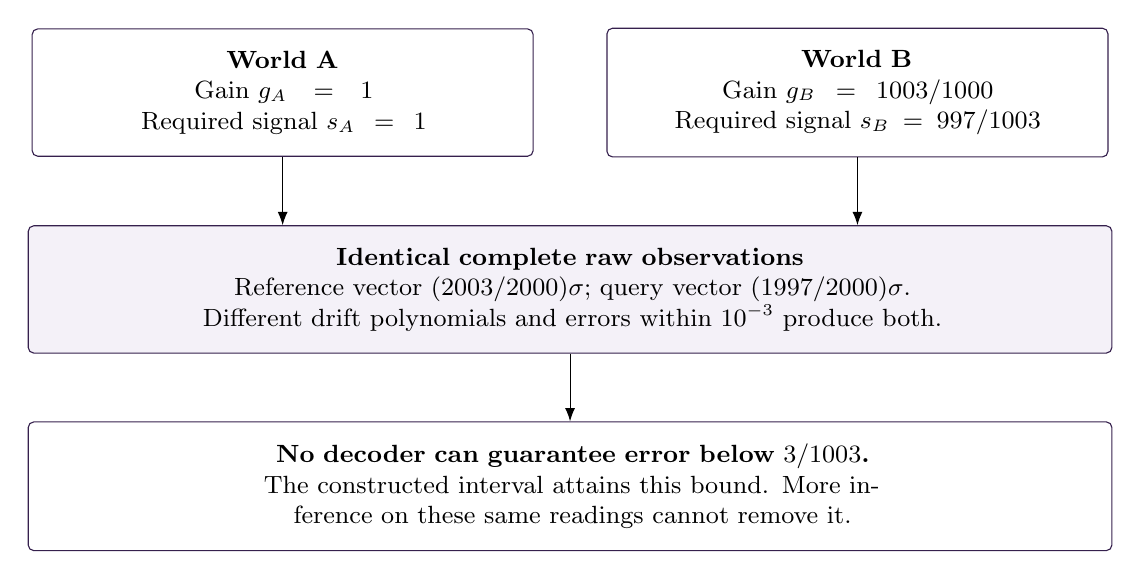
\begin{tikzpicture}[>=Latex,font=\small,box/.style={draw=ink,rounded corners=2pt,align=center,inner sep=8pt}]
\node[box,text width=5.8cm] (a) at (3.1,0) {\textbf{World A}\par Gain $g_A=1$\par Required signal $s_A=1$};
\node[box,text width=5.8cm] (b) at (10.4,0) {\textbf{World B}\par Gain $g_B=1003/1000$\par Required signal $s_B=997/1003$};
\node[box,fill=pale,text width=13.2cm] (same) at (6.75,-2.5) {\textbf{Identical complete raw observations}\par Reference vector $(2003/2000)\sigma$; query vector $(1997/2000)\sigma$.\par Different drift polynomials and errors within $10^{-3}$ produce both.};
\draw[->] (a.south)--(same.north -| a.south);
\draw[->] (b.south)--(same.north -| b.south);
\node[box,text width=13.2cm] (bound) at (6.75,-5.0) {\textbf{No decoder can guarantee error below $3/1003$.}\par The constructed interval attains this bound. More inference on these same readings cannot remove it.};
\draw[->] (same)--(bound);
\end{tikzpicture}
\caption{The primary sharp lower-bound witness. This is an exact synthetic pair, not two measured physical devices. It challenges every reconstruction rule under the specified model, including nonlinear ones.}
\label{fig:witness}
\end{figure}

\subsection{Fresh construction cases and adversarially valid observations}
After the implementation and independent checker were complete, final confirmation used seed 20261021431. The source and settings were hashed before the generated cases ran. The protocol is authored, not externally preregistered or blinded.

Forty-eight cases vary degree zero through three, available time slots, reading/switching/waiting prices, noise bounds and intended reuse. Their catalogues contain 1,764 informative programmes, each checked independently by a linear solve, moment cancellation, signal normalization and dual polynomial. Thirty-six cases admit the requested fixed-pair design. Twelve refuse it: their specified tolerance lies below the architecture's available noise floor. These counts reflect the chosen generator, not a success probability for real scientific work. Every reported choice is compared with exhaustive full-catalogue pairing; a refusal is not inferred merely from a search timeout.

\subsection{Adaptive repeated use under changing drift}
Twenty-four independent synthetic campaigns each acquire one numerical reference and then make 64 sequential queries. Their gains range over supplied positive rational values and are held fixed per campaign. Every block draws new polynomial coefficients and new componentwise errors. Drift magnitudes range over several orders, while the per-reading error contract remains unchanged. The next query's two design coordinates depend on the preceding reported midpoint, so the history is genuinely adaptive.

Every raw reading, coefficient, error, actual polarity and query is saved. The checker reconstructs the history without importing the constructor or forward-response module. All 1,536 response intervals contain the actual response. The largest observed midpoint error is approximately $0.00144304$, below the promised $1/334$ for the repeated-use design. The programme performs 6,144 raw query readings and 96 reference readings. Those counts are measurement settings in a simulator, not elapsed laboratory experiments.

A finite successful replay does not establish the all-history claim. The pathwise interval argument does, conditional on the common gain and each block's stated bounds. The result is not a probabilistic empirical claim that unmodeled drift never occurs.

\subsection{Two different decisions inherit the same calibrated interface}
The one-use primary programme is frozen and calibrated at synthetic gain $7/5$. It then serves two distinct response functions on $u,v\in\{0,1/19,\ldots,1\}$:
\begin{align}
 f_1(u,v)&=\frac12-\frac12(u-2/5)^2-\frac12(v-3/5)^2+\frac{uv}{20},\\
 f_2(u,v)&=u^3-v^2.
 \label{eq:functions}
\end{align}
Both lie in $[-1,1]$. These laws are supplied to the evaluator, not discovered natural laws or inputs to the programme compiler. New drift is generated for every call. Both decision procedures pay for actual observations of the full 400-point grid; a qualified interface is not an oracle that reveals unknown functions without queries.

For the first task, choose the grid point with the largest certified lower bound on $f_1$. The selected point is $(8/19,12/19)$. Its actual finite-grid regret is zero, but the earned certificate is the maximum competing upper endpoint minus its lower endpoint: approximately $0.00324086$. Overlapping intervals do not certify a unique optimum.

For the second task, select a point minimizing the certified distance of $f_2$ from $1/3$. The chosen point is $(14/19,5/19)$, with actual error $52/20577\approx0.00252709$ and certified error approximately $0.00424694$, below the separately declared tolerance $0.01$. Across both studies, all 800 response intervals contain the intended values. This is technical reuse across two decision requirements, not two physical discoveries or two operating businesses.

\begin{table}[htbp]\centering\small
\caption{New executed evidence. Counts overlap their constituent checks and must not be added as independent discoveries.}
\begin{tabularx}{\linewidth}{@{}YrY@{}}\toprule
Check & Count & Meaning\\\midrule
Canonical primary schedules & 448 & 380 informative, 68 aliases retained.\\
Full reference/query pairs & 144,400 & Exhaustive primary cost comparison.\\
Reuse horizons & 100 & Same accepted precision, different initial design.\\
Sharp complete-data witness pairs & 74 & Identical readings; attained half-separation.\\
Conditional-radius cases & 120 & Exact breakpoint verification.\\
General schedule certificates & 32 & Independent primal/dual checks.\\
Fresh finite construction cases & 48 & 36 qualifying, 12 refused.\\
Fresh informative programmes & 1,764 & Independent weights, moments and cost checks.\\
Adaptive response blocks & 1,536 & Exact replay across 24 campaigns.\\
Downstream response blocks & 800 & Maximization and inverse-target tasks.\\
New unit-test methods & 38 & Algebra, contracts, failures and mutations.\\\bottomrule
\end{tabularx}
\label{tab:evidence}
\end{table}

\section{A successor inherits valid evidence, not yesterday's scope}
\label{sec:successor}
A gain calibration can remain useful even when the query programme becomes invalid. The executed successor begins with degree-one drift and the three-reading programme
\begin{equation}
 t=(0,1,2),\quad\sigma=(+,-,+),\quad w=(1,-2,1)/4.
 \label{eq:linearprogramme}
\end{equation}
A valid historical reference at gain two yields the interval $[1.999,2.001]$. The original linear-drift query is correctly bounded.

Now the authorized query environment admits quadratic drift, while the same gain and valid historical reference are retained. Reusing (\ref{eq:linearprogramme}) on drift $7-3t+t^2$ and intended signal $1/4$ reports an interval near $1/2$; it misses the true response. The new compiler generates a four-reading degree-two programme. Using the \emph{same} gain evidence, its reported interval is
\begin{equation}
 \left[\frac{997}{4002},\frac{1003}{3998}\right],
 \label{eq:successorinterval}
\end{equation}
which contains $1/4$. The successor adds one reading per query and needs no new reference readings \emph{in this unchanged-gain example}. It does not pretend the earlier query programme was universally valid.

This is compatible inheritance, not automatic model repair. If the original reference itself had unknown quadratic drift when it was analyzed as linear, the old calibration would need revalidation from raw data or replacement. If gain changes, the old numerical interval is no longer evidence about the new gain. Both situations require a different continuation contract.

\subsection{Failures that define what has actually been learned}
\paragraph{A signal-shaped nuisance cannot be canceled while preserving the signal.}
An extra term $b\sigma$ is indistinguishable from a change in $gs$. Every valid contrast has $w^T\sigma=1$, so it passes that nuisance as well. The saved $b=1/10$ control produces a wrong nominal interval. A new sensor, reference structure or physical restriction is needed; more polynomial cancellation cannot solve the alias.

\paragraph{A higher-order drift can defeat a correct lower-order programme.}
The quadratic programme in (\ref{eq:primaryword}) does not annihilate cubic drift. The recorded coefficient $1/100$ on $t^3$ shifts its corrected product by $3/80$, exceeding the accepted error budget. If the additional drift is only approximately polynomial, a justified residual bound must be added to the per-reading error. A favorable fit on the same few observations does not establish that bound.

\paragraph{A gain change is not a new sign.}
The original finite paper's gain-two misspecification is now handled by numerical calibration when the gain remains stable. But a gain change \emph{after} calibration remains a real failure: using a unit-gain interval for a gain-two query produces an invalid result. A successor cannot inherit a physical equality merely because the software record persists.

\paragraph{Exact arithmetic is not infinite hardware dynamic range.}
With quadratic coefficients of order $10^{18}$, the saved rational example has exact contrast $1/4$, whereas converting its readings and weights to binary64 yields zero in the recorded run. This is an exposed numerical failure, not a claimed robust floating implementation. Quantization, saturation, timing and arithmetic error must fit the raw-error allowance, and sensor range must be sufficient. No theorem here cancels a clipped reading or restores information lost before acquisition.

\paragraph{More samples need not remove adversarial bias.}
The raw errors are bounded, not independent mean-zero draws. They may align with the contrast weights. Repetition can help under a justified stochastic or additional structural model, but no $1/\sqrt n$ claim follows from the present contract. The lower-bound witnesses exploit exactly this distinction.

\section{What survives from the original Out-Learn}
\label{sec:lineage}
The original paper asked how to combine evidence and persistent installations when recipe validity differs across a finite hypothesis class. It required \emph{one executable recipe that works across every survivor}, not a different hidden choice in each world. Its continuation theorem prices unresolved uncertainty across future compatible inheritance. Its finite minimax planner also retains a campaign-wide corrupted-reply budget, rather than resetting that budget after an inconvenient observation \cite{original}.

Those contributions are preserved, not declared superseded by a metrology example. Appendix~\ref{app:finite} restates the central identity with its proof and unchanged domain. The complete original PDF, LaTeX and executable companion are retained. In the present work the original source was inspected and rerun in a separate directory: all thirty tests passed, its saved-artifact checker passed, and nine deterministic JSON outputs matched byte-for-byte. This reproduces the original numerical study, not its physical premises or a new agent experiment.

The new results address a different missing layer. The earlier trusted bypass was supplied; the revised flagship constructs a drift-rejecting programme from reversal, timing and raw observation, then learns an unknown continuous gain. No finite table of possible gains or polynomial coefficients supplies the answer. The output changes from a policy over already-described useful components to a complete, costed experiment-and-calibration interface.

This is not a logical claim that the new model includes every original finite problem. Categorical lies and bounded numerical error are different evidence contracts. Submodular acquisition regret and minimax response error have different units. Their proper composition would first qualify a new measurement capability, then expose its true scope and costs to a higher-level planner. The present paper does not invent a single theorem by equating these distinct guarantees.

\section{Invent the economy of learning}
\label{sec:economy}
\subsection{A use commitment changes the experiment worth constructing}
The commercial implication is not an invoice attached to a faster calculation. Accepted precision and reuse scope change the measurement programme itself. In the primary model, $N\le18$ favors a modest calibration followed by the same modest query programme. At $N\ge20$, a more expensive, better-conditioned calibration supports cheaper future observations. That decision is made before the repeated work occurs.

This supplies a concrete connection to \emph{Invent the Economy}: beneficiaries, acceptance conditions, construction and reuse must be considered jointly \cite{economy}. A funded research or instrument organization might commission a qualified interface for repeated investigations. A single sponsor may suffice. Several users can share calibration only when they genuinely share the same stable gain, compatible instrument, capacity and permitted rights. Unrelated devices do not inherit a numerical calibration merely because they run the same software.

The proposed product is a qualified measurement capability: executable time/polarity programmes, traceable calibration evidence, numerical implementation, response intervals, supported nuisance class and a maintained requalification procedure. Customers should benefit when redundant fitting, sensing or reconstruction disappears. Continuing charges must support real maintenance and qualification, not preserve unnecessary agent activity.

\subsection{The resource frontier is not a business valuation}
For candidate programmes $p_c,p_o$ and a valid shared-use horizon, the experimental subtotal is $c_c+Nc_o$. A real offer also pays for modulation hardware, the reference standard, environmental control, domain expertise, discovery failures, independent checking, numerical validation, integration, downtime, maintenance, liability and financing. Those costs are not measured by the present rational computation.

Let $K$ be the complete shared construction and qualification cost, $a_j$ each use's full adaptation and operation cost, and $b_j$ the cost of a credible quality-matched alternative. A useful accounting condition is
\begin{equation}
 K+\sum_j a_j<\sum_j b_j.
 \label{eq:economic}
\end{equation}
It does not establish demand, consent or realized savings. A mature instrument, simultaneous reference channel, narrower drift model or more stable sensor may dominate the proposed programme after complete costs are included. No customer, quotation, success probability or sale is invented here.

A research agreement can purchase an honest investigation, including a valid negative result. Deployment acceptance separately requires the functioning apparatus and the promised range of measurements. Future receipts do not finance costs that must be paid first unless an actual authorized financing arrangement supplies usable resources. Refund and reserve obligations remain distinct from gross cash receipts. The same-plan cash-prefix warning in \emph{Out-Strategise} still applies \cite{strategise}.

MONTREAL.AI retains its parent ownership as a design constraint; project licenses or separately financed ventures require explicit agreements. Public linear algebra and open methods do not create exclusive rights by association. Where implementation uses the existing ecosystem, AGIJobManager's USDC route remains separate from the Alpha/Jobs v0 \$AGIALPHA routes. No token-holder equity, dividend or price entitlement is created by this paper.

\subsection{From one learned interface to a family of useful investigations}
\Om's intended durable asset is the programme plus its supported scope, valid calibration, failure record, real deployment rights and continuing economics. Alpha can develop the candidate construction; Jobs can commission bounded implementation and independent evaluation; Fleet can supply qualified execution and review. These are proposed integration roles, not a claim that this research package has been deployed into the live platform.

The productive sequence is concrete: qualify a measurement capability, validate a genuinely different use, obtain accepted delivery, retain surplus after obligations, and finance a separately qualified next construction. Better scientific, industrial or energy capabilities can build on such instruments. Every step requires evidence; a theoretical interface does not automatically supply a physical asset, paying demand or a self-accelerating economy.

\section{Nearest prior art and the boundary of the contribution}
\label{sec:prior}
\paragraph{Drift-rejecting measurement design.}
Doiron develops drift-eliminating non-simultaneous comparison calibrations \cite{doiron}. Swanson and Schlamminger construct filters for polynomial drift in alternating AB observations and analyze their statistical cost under uncorrelated stationary noise \cite{swanson}. These precedents are close and decisive: polarity reversal, polynomial cancellation and the value of calibration are not new discoveries here. Our design uses deterministic raw-error bounds, an explicit reading/switch/time cost, and an exact gain-calibration/query coupling. It does not claim those older methods are unable to be adapted to the same purpose.

\paragraph{Optimal recovery and interpolation.}
Ettehad and Foucart give computational optimal-recovery constructions for inaccurate observations under bounded error \cite{ettehad}. The quotient identity, interval midpoint and indistinguishable-world method belong to that tradition. Barycentric weights are established interpolation machinery \cite{berrut}. Our completed derivation makes these ingredients serve a specific constructed interface: a sparse acquisition optimum, its scoped adaptive lower bound, and the exact calibration--use radius in (\ref{eq:campaignrisk}). A focused review is not a proof of priority over every specialization of optimal recovery.

\paragraph{Experimental design and ratio estimation.}
Optimal-design work such as Sagnol's conic formulation selects informative experiments under its own observation and variance criteria \cite{sagnol}. Fieller's ratio-inference work concerns statistical uncertainty in numerator and denominator \cite{fieller}. We do not conflate those stochastic criteria with worst-case independent error boxes. The comparison here is between admissible schedules at the \emph{same deterministic precision}, with acquisition and reuse counted explicitly.

\paragraph{Purpose-sensitive learning and generated programmes.}
Decision-region determination learns enough to choose a valid decision without identifying every hypothesis \cite{javdani}; interactive submodular set cover unifies information acquisition with productive actions \cite{guillory}. These are already central credits in the original Out-Learn. AlphaEvolve generates and evaluates executable algorithm candidates \cite{alphaevolve}. Such a system could propose or optimize an experiment grammar, but no model system is run or defeated in the current study. The fact that a reference compiler returns a programme does not establish a learned improvement in how programmes are invented.

\paragraph{The supplied research lineage.}
\emph{Transformational Intelligence} supplies purpose-preserving reformulation \cite{transform}. \emph{Discoverability by Construction} makes missing measurement access an output \cite{discoverability}. \emph{The World as an Output} makes a nuisance-removing preparation programme an output \cite{world}. \emph{Out-Strategise} protects alternative enabling possibilities under future inheritance \cite{strategise}. This revision adds a numerical, continuous-uncertainty learning interface and sharp experiment/calibration guarantees. Earlier physical assumptions and theorem counts are not silently transferred to the new modality.

\section{The next decisive test and the earned conclusion}
\label{sec:conclusion}
The constructive achievement is a reproducible method that returns a measurement schedule, its exact correction and dual obstruction, a calibrated gain interval, and response bounds that survive new queries within scope. It can establish when more decoding cannot help; when a different acquisition programme can; when stronger calibration pays for reuse; and when a new nuisance class demands a new programme rather than another confidence label.

Its main limitation is now precise. The input assumptions---signal-preserving reversal, a suitable reference, stable gain, polynomial drift plus bounded residual, and enough dynamic range---must be established in the apparatus. The compiler learns numerical calibration but does not discover those physical laws from arbitrary data. Finite programme search remains combinatorial. The fixed-pair optimum is not a universal optimum over all hardware or adaptive unknown-gain experiments. The exact-rational implementation is not a production floating-point or hardware certificate.

A decisive next experiment would select a real drift-limited measurement independently of this method. It would compare a competent existing reversal/filtering design, a specialist numerical estimator, and the constructed protocol under the same purpose, hardware authority and full resource budget. Timing errors, gain drift, reference uncertainty, switching effects and saturation would be measured, not assumed away. A fresh response family and a changed drift scope would test transfer. That physical experiment remains unrun; it is not used as a substitute for the completed mathematics and executable study.

\thesis{\textbf{The strongest learning does not always leave a more elaborate explanation. It can leave a better way to obtain a trustworthy answer.}\par\smallskip
Construct the experiment. Learn what remains necessary. Preserve the evidence that lets the next discovery begin further ahead.}

\Needspace{5\baselineskip}
\noindent\textbf{Research status.} AI-assisted mathematics and exact synthetic computation. No physical qualification, comparative frontier-model trial, commercial exchange or external peer review is claimed. Proofs are not proof-assistant formalizations.

\appendix
\section{Duality, sparsity and the exact role of information}
\label{app:duality}
The finite contrast problem can be written as a linear programme in $w^+,w^-$ with objective $\mathbf1^T(w^++w^-)$ and equalities
\begin{equation}
 [\sigma\ \ V_d]^T(w^+-w^-)=(1,0,\ldots,0)^T.
\end{equation}
Its dual maximizes a scalar $\lambda$ subject to $\norm{\lambda\sigma+V_d\beta}_\infty\le1$. When $\sigma\notin\calV$, the optimum is $1/\kappa$ after rescaling a closest polynomial; it agrees with the geometric proof. The primal has an optimum because any finite objective level restricts $w$ to a compact set. A feasible basic optimum supplies the $d+2$ support bound. On fewer distinct points, the homogeneous Vandermonde equations force all weights to zero, contradicting signal normalization.

These statements require that raw reading error is bounded in infinity norm. Heterogeneous known bounds replace $\norm w_1$ by a weighted norm and require correspondingly modified formulas. A covariance matrix does not justify that substitution; it describes a different statistical objective. The present implementation uses one raw bound per programme and does not claim to solve every experimental-design criterion.

For the primary programme, $A=3/2$ and the dual polynomial is $p(t)=5/3-2t/3$. At the four selected slots its residual from the sign vector has maximum magnitude $2/3$. Thus $A\kappa=1$ exactly. The direct checker solves the moment/normalization system independently instead of calling the barycentric constructor. Its auxiliary Chebyshev checker solves candidate active-constraint systems and verifies all residual inequalities.

The adaptive theorem uses one fixed pair of worlds after the zero transcript has selected a schedule. It does not let an adversary change gain, signal or drift midway through a block. The constructed polynomial coefficients and errors reproduce every prefix, so the deterministic decision rule follows that same schedule in both worlds. Randomized algorithms are covered only if the guarantee is required pathwise for every realized seed; an expected-risk randomized theorem is not claimed.

No lower bound here denies richer observations. A simultaneous paired channel can remove a common nuisance with fewer distinct time samples. A known drift coefficient, a bounded coefficient set, an additional reference sensor, or a physically stable gain can reduce the required acquisition. Those are changes to the available information or apparatus and should be compared at their actual cost.

\section{Sharp calibrated recovery and full-data witnesses}
\label{app:witness}
\subsection{The conditional radius in three regimes}
Equation~(\ref{eq:conditionalrisk}) is equivalently
\begin{equation}
R(a,b,e,S)=
\begin{cases}
 [S(b-a)+2e]/(2b), & 0\le e\le aS/2,\\
 e/a, & aS/2\le e\le aS,\\
 S, & e\ge aS.
\end{cases}
\end{equation}
In the first regime the indistinguishable endpoints can be chosen as $s_A=S$ at gain $a$ and $s_B=(aS-2e)/b$ at gain $b$, with common $z=aS-e$. In the middle regime use gains $a$ and signals $\pm e/a$ with $z=0$. In the last use signals $\pm S$. These witnesses show why an upper bound based only on first-order ratio error is not the sharp answer.

A pointwise clipped interval can be much tighter than the global worst case. The global radius is a guaranteed supremum before the observations arrive, not a claim that every query realizes that error. Conversely, selecting favorable observed values cannot shrink a published worst-case guarantee without changing its quantifier.

\subsection{Primary campaign numbers}
For $e_c=e_o=3/2000$, $g_0=S=1$, the two worlds are
\begin{equation}
(g_A,s_A)=(1,1),\qquad(g_B,s_B)=(1003/1000,997/1003).
\end{equation}
They have common reference vector $(2003/2000)\sigma$ and common query vector $(1997/2000)\sigma$. Use $p(t)=5/3-2t/3$ in the signed nuisance/error construction of Theorem~\ref{thm:campaign}. The raw noise equals $\pm1/1000$ at the appropriate coordinates. Every reading is shared, and the half signal separation is $3/1003$.

The same argument works with different optimal reference and query programmes. In the repeated-use optimum, $e_c=1/1000$ and $e_o=2/1000$, giving radius $1/334$. The stored witness includes all coefficients, gains, signals and individual raw errors for both worlds. A separate interpreter verifies equal complete observation vectors rather than only equal contrasts.

If no numerical reference is acquired and only $g\ge g_0$ is known, the exact supremal radius after a drift-rejected product with error $e$ is
\begin{equation}
 R_{\rm no\ ref}=\min\{S,\max\{S/2,e/g_0\}\}.
\end{equation}
For positive products bounded away from zero, the feasible positive signal approaches zero as gain grows without bound; a product compatible with $s=S$ therefore gives width approaching $S$. At zero product, the feasible interval has radius $\min\{S,e/g_0\}$. These cases also bound every other product. This is an explicit comparator: the tight primary tolerance cannot be met by silently treating an uncalibrated gain as known.

\subsection{What is and is not optimal over an entire history}
The fixed-pair minimax law permits arbitrary independent nuisance coefficients in the reference and query blocks. It does not assume that the same polynomial spans the two blocks. A design that intentionally enforces such shared drift may use more information, but must establish that stronger contract.

The returned reference interval remains valid on later uses. Observing many bounded signals can sometimes shrink the set of gains consistent with the full history. The current decoder does not exploit that possibility and is not called full-history minimax. Likewise, it does not optimize the number of reference blocks, adapt calibration precision to observed gain, or solve arbitrary recurrent calibration scheduling. Those are specific extensions, not hidden capabilities of the two-block theorem.

\section{The inherited continuation theorem, preserved at its own strength}
\label{app:finite}
The original Out-Learn model uses a finite hypothesis set $H$, compatible durable capabilities $M$, and executable recipes $p$ with requirements $K_p\subseteq M$ and validity region $\Gamma_p\subseteq H$. For survivors $V$, let $A(V)$ be the minimal requirement sets of recipes whose \emph{same implementation} works for every $h\in V$. Let $A_h=A(\{h\})$. A normalized monotone submodular acquisition cost $C$ gives marginal $D_C(T\mid I)=C(I\cup T)-C(I)$.

With installed assets $I$, define
\begin{equation}
 L(V,I)=\max_{h\in V}\max_{J\supseteq I}
 \left[\min_{T\in A(V)}D_C(T\mid J)-\min_{S\in A_h}D_C(S\mid J)\right].
\end{equation}
For nonempty relevant recipe families, the inherited identity is
\begin{equation}
 L(V,I)=\max_{h\in V}\max_{S\in A_h}\min_{T\in A(V)}
 \big[C(I\cup S\cup T)-C(I\cup S)\big].
 \label{eq:inherited}
\end{equation}
For completeness, fix $h,J$ and an informed optimizer $S$. A common $T$ covering it on the right satisfies
\begin{align*}
 D_C(T\mid J)&\le D_C(S\cup T\mid J)\\
 &=D_C(S\mid J)+D_C(T\mid J\cup S)\\
 &\le D_C(S\mid J)+D_C(T\mid I\cup S).
\end{align*}
This gives the upper bound. For a maximizing informed pair $(h_*,S_*)$, take $J=I\cup S_*$. Informed acquisition is zero and common acquisition attains the claimed right-hand value. This proves equality. The mathematical engine is the prior Out-Strategise continuation identity, credited rather than introduced again \cite{strategise,original}.

The original learner chooses between persistent installations and observations. A capped mismatch vector preserves each hypothesis's consumed share of a global categorical-corruption budget. Positive-cost probes with a feasible identical-state branch can be omitted for its stationary minimax objective; the remaining state progression is acyclic and exact dynamic programming applies. Its programme and thirty-test study are retained in the original companion, including pairwise/common-recipe failures and scope-changing successor accounting.

The present revision does not reinterpret $L$ as numerical measurement error. A zero value of $L$ means no additional acquisition disadvantage relative to an informed investigator under the declared compatible future contexts. It does not prove physical installation or zero response error. Conversely, a small radius in (\ref{eq:campaignrisk}) does not establish acquisition optimality, financing or future recipe compatibility. Keeping these units and claims separate is necessary for meaningful integration.

\section{Reproducibility, actual inputs and complete work accounting}
\label{app:reproduce}
\subsection{Exact reference implementation}
The new code uses only Python's standard library. The final run uses Python 3.13.5 in the recorded Linux container; the environment record is authoritative if a later reproduction uses a different version. All scientific arithmetic in the constructor, simulator and checker is integer or rational. Binary64 is used only in a separately labelled numerical-failure control and descriptive elapsed-time reporting.

From the extracted package root, run:
\begin{verbatim}
python code/run_study.py --out rerun
python code/check_artifacts.py --results rerun
python -m unittest discover -s code -p 'test_*.py' -v
pdflatex -no-shell-escape -interaction=nonstopmode \
  -halt-on-error -output-directory=paper paper/Out_Learn_Revised.tex
pdflatex -no-shell-escape -interaction=nonstopmode \
  -halt-on-error -output-directory=paper paper/Out_Learn_Revised.tex
\end{verbatim}
The driver refuses to overwrite a nonempty result directory. The manuscript contains all figures and references; it needs no network fetch, shell escape or separate graphics files. Ordinary installed TeX packages are required. No font files are redistributed.

\begin{table}[htbp]\centering\small
\caption{Principal new artifacts. The independent checker imports only its own reference arithmetic, not the constructor or forward laboratory.}
\begin{tabularx}{\linewidth}{@{}P{.43\linewidth}Y@{}}\toprule
Path & Role\\\midrule
\path{code/experiment.py} & Programme synthesis, interval learning, exact risk and pair selection.\\
\path{code/laboratory.py} & Synthetic black-box observations and sharp complete-data witnesses.\\
\path{code/reference.py} & Separate elimination, primal verification and observation replay.\\
\path{code/check_artifacts.py} & Saved catalogue, optimality, witness and full-history verification.\\
\path{code/test_experiment.py} & Thirty-eight boundary, mutation and negative-control tests.\\
\path{results/final/primary.json} & All 448 primary candidates, frontier, 100 horizons and worked example.\\
\path{results/final/theorem_checks.json} & Conditional radii, generic schedules and raw lower-bound pairs.\\
\path{results/final/confirmation.json} & Forty-eight complete synthetic construction cases.\\
\path{results/final/adaptive.json} & Every calibration and query reading across 24 histories.\\
\path{results/final/applications.json} & Eight hundred observed responses and both decision records.\\
\path{results/final/scope_and_failures.json} & Actual successor, invalid scopes and numerical failure.\\
\path{provenance/inherited_reproduction.json} & Nine original output hashes and separate rerun evidence.\\\bottomrule
\end{tabularx}
\end{table}

\subsection{Generated inputs and evidence separation}
The final seed is 20261021431. The generator uses offsets $+1,+3,+5,+7$ for theorem checks, fresh construction cases, adaptive campaigns and downstream grids. In case $i=0,\ldots,47$, degree is $i\bmod4$, slot count is $d+2+(i\bmod3)$, and the tolerance is the noise bound multiplied by $1,2,3,$ or $5$ according to $i\bmod4$. Reading prices are integers one through three, switching prices zero through four, and waiting prices zero through $3/10$. Thus the twelve deliberate low-tolerance cases test refusal; their frequency is not a scientific population estimate.

Adaptive gain is $1+k/17$ for a generated integer $k\in\{0,\ldots,60\}$. Each block generates fresh rational polynomial coefficients and errors in the stated box. Its next coordinates depend on the previous midpoint through an explicitly recorded finite-grid transformation; the exact formulas and every realized value are in the code and output. The checker recomputes both the adaptation and the actual polarity carried across blocks. Only the evaluator and checker receive the true gain, drift and responses.

The two downstream laws are evaluated on all 400 grid points each. Selection uses returned intervals, not hidden true values. The independent checker expands $f_1$ as
\begin{equation}
 f_1(u,v)=\frac6{25}-\frac{u^2}{2}+\frac{2u}{5}-\frac{v^2}{2}+\frac{3v}{5}+\frac{uv}{20},
\end{equation}
and separately verifies the maximization and inverse-target conclusions. No finite-grid result is presented as an optimum over the unqueried continuum.

\subsection{Development, search cost and reproduction}
A preliminary run used seed 20261021413. Its results are retained, but no full source snapshot for that intermediate version is claimed. A checked development version, with its source, used seed 20261021419. The final version added the explicit contract fields, independent checker and complete tests before running the fresh final seed. The physical model, primary costs and accepted error were unchanged. These are authored development records, not external preregistration.

The experiment ledger counts all raw readings in each selected protocol. The constructor additionally evaluates rejected schedules, alternative programme pairs and failed tolerances. Its verification deliberately spends extra computation to inspect every candidate and saved observation. The recorded final driver runtime is a single local measurement, not a benchmark against an inventor or a physical laboratory. Literature search, derivation, AI-assisted programming, review, actual energy and hardware qualification are not comprehensively metered and are not zero costs.

The original Out-Learn package is preserved unchanged. Its separate rerun reproduces nine deterministic files and thirty passing tests. New deterministic outputs, source identities and test logs are retained separately; environment timing is excluded from byte-identical scientific reproduction claims. Hashes identify bytes, not the truth of a physical assumption.

\Needspace{13\baselineskip}
\section{Claim--evidence register and scope}
\label{app:claims}
\small
\begin{longtable}{@{}P{.28\linewidth}P{.34\linewidth}P{.32\linewidth}@{}}\toprule
Claim & Evidence & Principal boundary\\\midrule\endfirsthead
\toprule Claim & Evidence & Principal boundary\\\midrule\endhead
Exact known-gain error & Theorem~\ref{thm:known}; primal/dual certificates and two-world construction & Unrestricted polynomial nuisance, bounded raw errors, fixed signal per block.\\[4pt]
$d+2$ samples suffice for cost optimum & Theorem~\ref{thm:sparse}; full primary catalogue & Distinct slots and deletion-monotone read/switch/time cost; not all sensor architectures.\\[4pt]
Adaptation cannot lower worst acquisition cost & Theorem~\ref{thm:adaptive}; zero-transcript proof & Deterministic, known gain, specified symmetric class; no general adaptive-learning claim.\\[4pt]
Exact learned calibration and response interval & Lemma~\ref{lem:sufficient}; raw-data replay & Sparse blocks; one valid reference; stable common gain.\\[4pt]
Sharp calibration--use minimax law & Theorems~\ref{thm:conditional}--\ref{thm:campaign}; 74 full-data pairs & Fixed separate-block programmes; all decoders, but not every adaptive calibration design.\\[4pt]
Reuse changes the reference worth acquiring & Corollary~\ref{cor:pair}; 144,400 pairs and 100 horizons & Supplied resource prices; compatible repeated scope; no commercial commitments.\\[4pt]
Adaptive repeated response validity & 1,536 saved query blocks; exact checker & Synthetic histories within the assumptions, not their physical justification.\\[4pt]
Different downstream purposes reuse one interface & Maximization and inverse-target studies, 800 response blocks & Authored function class; no independent natural discovery or commercial adoption.\\[4pt]
A scope-changing successor reuses valid gain evidence & Linear-to-quadratic case with failed old query and corrected new one & Same true gain, valid historical calibration; changed past semantics require revalidation.\\[4pt]
Original finite learner remains reproducible & Nine original JSON byte matches; thirty tests & Its finite catalogue and supplied bypass remain its scope.\\[4pt]
A newly viable business or superior invention policy & Not established & Requires external qualification, matched discovery campaigns and actual accepted economics.\\\bottomrule
\end{longtable}
\normalsize

\section{Sources and research transparency}
The supplied Out-Learn PDF, LaTeX, complete computational package and review notes were inspected. Its computations were rerun rather than promoted from manuscript claims to new evidence by repetition. The supplied preceding papers identify the programme's lineage; their exact local identities are recorded, and their older computations are not claimed as newly reproduced here. No mutable repository link is treated as proof of a current release.

Primary manuscripts and publisher records were inspected through 21 October 2026. The source ledger distinguishes mathematical-text inspection from abstract/metadata checks. Established drift rejection, optimal recovery and purpose-sensitive learning are credited; no exhaustive priority or external peer-review claim is made. Original sources and operational systems remain unchanged. All new work is local, analytical or synthetic.

\clearpage
\begin{thebibliography}{99}
\small\raggedright
\bibitem{original} Vincent Boucher. \emph{Out-Learn: Change What You Need to Know. Continuation-Sufficient Learning through Evidence and Construction}. Original 23-page research manuscript and executable companion, 21 October 2026. Preserved unchanged in the revision package; source identities and rerun records supplied.
\bibitem{transform} Vincent Boucher. \emph{Transformational Intelligence: Learning to Change the Game}. MONTREAL.AI research manuscript, October 2026. Supplied foundation. \url{https://github.com/MontrealAI/AGI-Alpha-Agent-v0/blob/main/docs/Transformational_Intelligence.pdf}.
\bibitem{economy} Vincent Boucher. \emph{Invent the Economy: Transformational Intelligence for Creating Viable Markets}. MONTREAL.AI research manuscript, October 2026. Supplied foundation. \url{https://github.com/MontrealAI/AGI-Alpha-Agent-v0/blob/main/docs/Invent_the_Economy.pdf}.
\bibitem{discoverability} Vincent Boucher. \emph{Discoverability by Construction: Synthesizing Experimental Access, Optimal Calibration, and Successor Capabilities}. Supplied research manuscript, 20 October 2026. Exact source identity retained.
\bibitem{world} Vincent Boucher. \emph{The World as an Output: Constructive Sufficiency for Reusable Discovery}. MONTREAL.AI research manuscript, 20 October 2026. \url{https://github.com/MontrealAI/AGI-Alpha-Agent-v0/blob/main/docs/The_World_as_an_Output.pdf}.
\bibitem{strategise} Vincent Boucher. \emph{Out-Strategise: Change What Winning Depends On}. Revised 25-page manuscript, 20 October 2026. Supplied source; exact identity retained.
\bibitem{doiron} Ted Doiron. Drift eliminating designs for non-simultaneous comparison calibrations. \emph{Journal of Research of the National Institute of Standards and Technology}, 98(2):217--224, 1993. \url{https://doi.org/10.6028/jres.098.016}. Open text: \url{https://pmc.ncbi.nlm.nih.gov/articles/PMC4909179/}.
\bibitem{swanson} H. Erik Swanson and Stephan Schlamminger. \emph{Removal of zero-point drift from AB data and the statistical cost}. arXiv:1009.1894v1, 9 September 2010. \url{https://arxiv.org/abs/1009.1894}.
\bibitem{ettehad} Mahmood Ettehad and Simon Foucart. Instances of computational optimal recovery: Dealing with observation errors. \emph{SIAM/ASA Journal on Uncertainty Quantification}, 9(4):1438--1456, 2021. \url{https://doi.org/10.1137/20M1328476}. Open manuscript: \url{https://arxiv.org/abs/2004.00192}.
\bibitem{berrut} Jean-Paul Berrut and Lloyd N. Trefethen. Barycentric Lagrange interpolation. \emph{SIAM Review}, 46(3):501--517, 2004. \url{https://doi.org/10.1137/S0036144502417715}.
\bibitem{fieller} E. C. Fieller. Some problems in interval estimation. \emph{Journal of the Royal Statistical Society, Series B}, 16(2):175--185, 1954. \url{https://doi.org/10.1111/j.2517-6161.1954.tb00159.x}.
\bibitem{sagnol} Guillaume Sagnol. \emph{Computing optimal designs of multiresponse experiments reduces to second-order cone programming}. arXiv:0912.5467v3, 25 November 2010. \url{https://arxiv.org/abs/0912.5467v3}.
\bibitem{javdani} Shervin Javdani, Yuxin Chen, Amin Karbasi, Andreas Krause, Drew Bagnell and Siddhartha Srinivasa. Near optimal Bayesian active learning for decision making. \emph{AISTATS}, PMLR 33:430--438, 2014. \url{https://proceedings.mlr.press/v33/javdani14.html}.
\bibitem{guillory} Andrew Guillory and Jeff Bilmes. \emph{Interactive Submodular Set Cover}. arXiv:1002.3345v2, 20 May 2010. \url{https://arxiv.org/abs/1002.3345}.
\bibitem{alphaevolve} Alexander Novikov et al. \emph{AlphaEvolve: A coding agent for scientific and algorithmic discovery}. arXiv:2506.13131v1, 16 June 2025. \url{https://arxiv.org/abs/2506.13131v1}.
\end{thebibliography}
\end{document}
